\documentclass[a4paper,12pt,titlepage]{report}
\usepackage{fontspec}
\defaultfontfeatures{Ligatures=TeX}
\IfFontExistsTF{Times New Roman}{\setmainfont{Times New Roman}}{\setmainfont{Liberation Serif}}
\usepackage[main=russian,english]{babel}
\usepackage{amsmath,amssymb,graphicx,geometry,setspace,indentfirst,titlesec,enumitem,caption,float}
\graphicspath{{figure/}{./}}
\geometry{left=2.5cm,right=1.5cm,top=2cm,bottom=2cm}
\titleformat{\chapter}[display]{\centering\bfseries}{ГЛАВА \thechapter}{8pt}{\MakeUppercase}
\titleformat{\section}{\normalsize\bfseries}{\thesection.}{1em}{}
\titlespacing*{\chapter}{0pt}{-20pt}{12pt}
\titlespacing*{\section}{0pt}{1.5\baselineskip}{.5\baselineskip}
\setcounter{tocdepth}{1}
\addto\captionsrussian{\renewcommand{\contentsname}{Содержание}}
\DeclareCaptionLabelSeparator{gost}{. }
\captionsetup{labelsep=gost,font=small}
\setlist{nosep}
\counterwithout{equation}{chapter}
\counterwithout{figure}{chapter}
\begin{document}
\singlespacing
\begin{titlepage}

\begin{center}

% Логотип временно выключен, чтобы сборка не зависела
% от формата изображения. Для XeLaTeX используйте PDF или PNG:
%

\includegraphics[width=0.8cm]{logo_unn}\par
\vspace{0.5em}

МИНИСТЕРСТВО НАУКИ И ВЫСШЕГО ОБРАЗОВАНИЯ\\
РОССИЙСКОЙ ФЕДЕРАЦИИ

\vspace{1em}

Федеральное государственное автономное образовательное учреждение\\
высшего образования

\vspace{0.5em}

\textbf{<<Национальный исследовательский\\
Нижегородский государственный университет им. Н.\,И.~Лобачевского>>}

\vspace{2em}

\textbf{Институт информационных технологий, математики и механики}

\vspace{2em}

Направление подготовки: <<Прикладная математика\\
и информатика>>

\end{center}

\vspace{1em}

\begin{center}
{\Large\bfseries
Отчёт по лабораторной работе №\,4\\
по уравнениям математической физики
}
\end{center}

\vspace{2.5em}

\begin{center}
{\large\bfseries Тема:}

\vspace{0.5em}

{\large\bfseries
<<Распространение тепла в конечном стержне>>
}
\end{center}

\vspace{4em}

\hfill
\begin{minipage}[t]{0.42\linewidth}
\raggedright

Выполнили:\\
студенты группы 3823Б1ПМоп2\\
Золкин Иван Александрович\\
Носов Владимир Михайлович

\vspace{1.5em}

Проверил:\\
к.\,ф.-м.\,н., доцент\\
Муняев Вячеслав Олегович

\end{minipage}

\vfill

\begin{center}
Нижний Новгород\\
2026
\end{center}

\end{titlepage}
\setcounter{page}{2}
\onehalfspacing\setlength{\parindent}{1.25cm}
\tableofcontents
\chapter{Теоретическая часть}
\section{Вывод уравнения теплопроводности и граничных условий}\label{sec:deriv}
Рассмотрим тонкий однородный стержень длины $l$, расположенный вдоль оси $Ox$, с постоянным поперечным сечением площади $S$ и периметром сечения $P$. Стержень тонкий, поэтому температуру во всех точках сечения считаем одинаковой и равной $u(x,t)$. Обозначим: $\rho$~--- плотность, $c$~--- удельная теплоёмкость, $k$~--- коэффициент теплопроводности, $F(x,t)$~--- плотность тепловых источников, $u_{\text{ср}}(x,t)$~--- температура окружающей среды, $h$~--- коэффициент теплообмена с окружающей средой.

\textbf{Уравнение.} Выделим малый участок стержня между сечениями $x$ и $x+\Delta x$ и составим для него баланс тепла за время от $t$ до $t+\Delta t$.

Количество тепла в участке равно $c\rho S\Delta x\,u$, поэтому его изменение
\[
\Delta Q=c\rho S\Delta x\bigl(u(x,t+\Delta t)-u(x,t)\bigr)\approx c\rho S\,u_t\,\Delta x\,\Delta t .
\]

Поток тепла вдоль оси по закону Фурье равен $q(x,t)=-k\,u_x(x,t)$. Через сечение $x$ в участок входит тепло $q(x,t)S\Delta t$, через сечение $x+\Delta x$ выходит $q(x+\Delta x,t)S\Delta t$. Приток тепла через сечения
\[
Q_1=S\bigl(q(x,t)-q(x+\Delta x,t)\bigr)\Delta t\approx -S\,q_x\,\Delta x\,\Delta t=kS\,u_{xx}\,\Delta x\,\Delta t .
\]

Через боковую поверхность участка (стенки) площадью $P\Delta x$ происходит теплообмен со средой по закону Ньютона: поток пропорционален разности температур стержня и среды. Теплота, полученная участком от среды,
\[
Q_2=-h\bigl(u-u_{\text{ср}}\bigr)P\,\Delta x\,\Delta t .
\]

Тепло, выделенное источниками, равно $Q_3=F\,S\,\Delta x\,\Delta t$.

Приравнивая $\Delta Q=Q_1+Q_2+Q_3$, деля на $c\rho S\Delta x\Delta t$ и устремляя $\Delta x,\Delta t\to0$, получаем
\[
u_t=\frac{k}{c\rho}u_{xx}-\frac{hP}{c\rho S}\bigl(u-u_{\text{ср}}\bigr)+\frac{F}{c\rho},
\]
то есть уравнение задачи
\[
u_t=a^2u_{xx}-bu+f(x,t),\qquad a^2=\frac{k}{c\rho},\quad b=\frac{hP}{c\rho S},\quad f=\frac{F}{c\rho}+b\,u_{\text{ср}} .
\]
Если боковая поверхность теплоизолирована, то $h=0$ и $b=0$.

\textbf{Граничные условия.} Граничные условия имеют вид
\[
\alpha u(0,t)-\beta u_x(0,t)=\mu(t),\qquad \gamma u(l,t)-\delta u_x(l,t)=\nu(t).
\]

\emph{Торец $x=0$ (I род).} На торце поддерживается заданная температура: $u(0,t)=\mu(t)$, т.\,е. $\alpha=1$, $\beta=0$.

\emph{Торец $x=l$ (II род).} Через торец наружу уходит заданный тепловой поток $q_l(t)$. Рассмотрим малый участок $[l-\Delta x,l]$ у торца: через сечение $l-\Delta x$ в него входит поток $q(l-\Delta x,t)$, через торец уходит $q_l(t)$:
\[
c\rho S\Delta x\,u_t\,\Delta t=\bigl(q(l-\Delta x,t)-q_l(t)\bigr)S\Delta t+O(\Delta x)\Delta t .
\]
При $\Delta x\to0$ получаем $q(l,t)=q_l(t)$, т.\,е. $-k\,u_x(l,t)=q_l(t)$. Деля на $k$, получаем $\gamma=0$, $\delta=1$, $\nu(t)=q_l(t)/k$. При $\nu=0$ торец теплоизолирован.

Итак, задача имеет вид
\[
\begin{cases}
u_t=a^2u_{xx}-bu+f(x,t),\quad 0<x<l,\ t>0, & u(x,0)=\varphi(x),\\
u(0,t)=\mu(t), & -u_x(l,t)=\nu(t),
\end{cases}
\]
где $\mu(t)=A\cos(\omega_1t)+B\sin(\omega_2t)$, $\nu(t)=0$.

\section{Функция Грина и её физический смысл}\label{sec:green}
Рассмотрим задачу с однородными граничными условиями и без источников:
\[
u_t=a^2u_{xx}-bu,\qquad u(x,0)=\varphi(x),\qquad u(0,t)=0,\qquad u_x(l,t)=0 .
\]
Решаем методом Фурье: ищем решения вида $u(x,t)=X(x)T(t)$. Подставляя в уравнение и разделяя переменные, получаем
\[
\frac{T'+bT}{a^2T}=\frac{X''}{X}=-\lambda^2,\qquad X''+\lambda^2X=0,\quad X(0)=0,\quad X'(l)=0 .
\]
Из $X(0)=0$ следует $X=\sin\lambda x$, а из $X'(l)=0$~--- $\cos\lambda l=0$. Отсюда
\[
\lambda_n=\frac{(2n-1)\pi}{2l},\qquad X_n(x)=\sin \lambda_nx,\qquad n=1,2,\dots,
\]
\[
T_n(t)=A_ne^{-(a^2\lambda_n^2+b)t},\qquad \|X_n\|^2=\int_0^l\sin^2\lambda_nx\,dx=\frac l2 .
\]
Ряд $u=\sum A_ne^{-(a^2\lambda_n^2+b)t}\sin \lambda_nx$ удовлетворяет начальному условию при
\[
A_n=\frac2l\int_0^l\varphi(\xi)\sin \lambda_n\xi\,d\xi .
\] Подставляя $A_n$ и меняя порядок суммирования и интегрирования, получаем
\[
u(x,t)=\int_0^lG(x,\xi,t)\varphi(\xi)\,d\xi,\qquad
G(x,\xi,t)=\frac2l\sum_{n=1}^{\infty}e^{-(a^2\lambda_n^2+b)t}\sin \lambda_nx\,\sin \lambda_n\xi .
\]

\textbf{Физический смысл.} Если $\varphi(x)=\delta(x-\xi)$, то $u=G(x,\xi,t)$. Значит, $G(x,\xi,t)$~--- температура в точке $x$ в момент $t$, если в начальный момент в точке $\xi$ мгновенно выделилось количество тепла $c\rho S$ (мгновенный точечный источник), левый торец поддерживается при нулевой температуре, правый теплоизолирован, а на боковой поверхности идёт теплообмен со средой нулевой температуры. Тепло, выделившееся в точке $\xi$ в момент $\tau$, даёт вклад $G(x,\xi,t-\tau)$, поэтому через $G$ выражается и действие источников $f$. При этом $G(0,\xi,t)=0$, $G_x(l,\xi,t)=0$, $G(x,\xi,t)\to\delta(x-\xi)$ при $t\to+0$, а $\int_0^lG\,dx$~--- доля тепла, оставшаяся в стержне к моменту $t$.

\textbf{График.} Построим $G$ при $l=1$, $a=1$, $b=0$, $\xi=0.3$ для $t_1=0.005<t_2=0.03$, суммируя первые 400 членов ряда (рис.~\ref{fig:green}).
\begin{figure}[H]
\centering
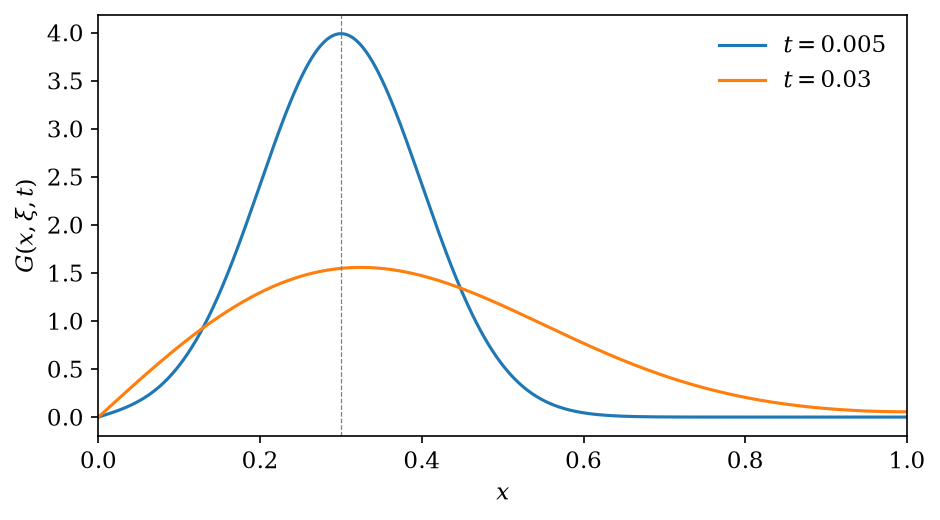
\includegraphics[width=0.75\textwidth]{green}
\caption{Функция Грина $G(x,0.3,t)$ при $t_1=0.005$ и $t_2=0.03$}
\label{fig:green}
\end{figure}
При $t_1$ функция Грина~--- узкий высокий пик в точке $\xi$ (максимум $\approx3.99$), близкий к фундаментальному решению на прямой: тепло ещё не дошло до торцов. При $t_2$ пик ниже ($\approx1.56$) и шире, его вершина смещена вправо ($x\approx0.32$): через левый торец тепло уходит, а правый торец теплоизолирован. Количество тепла в стержне уменьшается: $\int_0^1G\,dx\approx0.997$ при $t_1$ и $\approx0.779$ при $t_2$. При $t\to\infty$ функция $G\to0$.

\section{Стационарный режим}
Пусть $f=f(x)$, $\mu=\mu_0$, $\nu=\nu_0$ не зависят от времени. \textbf{Стационарным режимом} называется не зависящее от времени распределение температуры $U(x)$, к которому стремится решение: $U(x)=\lim_{t\to\infty}u(x,t)$. Подставляя $u=U(x)$ в задачу, получаем краевую задачу для $U$:
\[
a^2U''-bU+f(x)=0,\qquad U(0)=\mu_0,\qquad -U'(l)=\nu_0 .
\]
Положим $u=U+v$. Функция $v$ решает однородную задачу
\[
v_t=a^2v_{xx}-bv,\qquad v(0,t)=0,\qquad v_x(l,t)=0,\qquad v(x,0)=\varphi(x)-U(x),
\]
поэтому
\[
v(x,t)=\int_0^lG(x,\xi,t)\bigl(\varphi(\xi)-U(\xi)\bigr)d\xi .
\]
Каждый член ряда для $G$ содержит множитель $e^{-(a^2p_n^2+b)t}$, где $a^2p_n^2+b>0$, поэтому $v\to0$ и $u\to U$.

\textbf{Неоднородность уравнения} $f(x)$ (источники и температура среды) входит в уравнение для $U$ и определяет форму стационарного профиля. Если $f$ зависит от $t$, стационарного режима, вообще говоря, нет.

\textbf{Начальные условия} в задачу для $U$ не входят и на стационарный режим не влияют: от $\varphi$ зависит только затухающая часть $v$. Исключение~--- случай $b=0$ с теплоизолированными обоими торцами: тогда есть собственное значение $\lambda_0=0$, слагаемое с $e^{0\cdot t}$ не затухает и стационарная температура равна среднему значению $\varphi$ (практическая задача 1).

\textbf{Неоднородности граничных условий} $\mu_0,\nu_0$ входят в граничные условия для $U$ и вместе с $f$ полностью определяют стационарный режим; при $f=0$ и однородных граничных условиях $U\equiv0$. Если $\mu$ или $\nu$ зависят от времени, стационарного режима нет, а при больших $t$ температура следует за изменением граничных условий (практическая задача 3).

\chapter{Практическая часть}
\section{Задача 1}
Боковая поверхность теплоизолирована и источников нет, поэтому $b=0$, $f=0$:
\[
u_t=a^2u_{xx},\qquad u(x,0)=x .
\]
Выберем однородные граничные условия II рода (теплоизолированные торцы):
\[
u_x(0,t)=0,\qquad u_x(l,t)=0 .
\]

Решаем методом Фурье. Задача $X''+\lambda X=0$, $X'(0)=X'(l)=0$ даёт
\[
\lambda_n=\Bigl(\frac{\pi n}{l}\Bigr)^2,\qquad X_n=\cos\frac{\pi nx}{l},\qquad n=0,1,2,\dots,
\]
\[
u(x,t)=\frac{A_0}2+\sum_{n=1}^{\infty}A_ne^{-\left(\frac{\pi na}{l}\right)^2t}\cos\frac{\pi nx}{l},\qquad A_n=\frac2l\int_0^l\varphi(x)\cos\frac{\pi nx}{l}\,dx .
\]
Для $\varphi(x)=x$:
\[
A_0=\frac2l\int_0^lx\,dx=l,\qquad A_n=\frac2l\int_0^lx\cos\frac{\pi nx}{l}\,dx=\frac{2l\bigl((-1)^n-1\bigr)}{\pi^2n^2},
\]
\[
u(x,t)=\frac l2-\frac{4l}{\pi^2}\sum_{m=0}^{\infty}\frac{1}{(2m+1)^2}\,e^{-\left(\frac{(2m+1)\pi a}{l}\right)^2t}\cos\frac{(2m+1)\pi x}{l}.
\]
Все слагаемые с $n\ge1$ затухают, поэтому $u\to l/2\ne0$ (рис.~\ref{fig:p1}).

При произвольном $\varphi$ стационарный режим равен
\[
U=\frac{A_0}{2}=\frac1l\int_0^l\varphi(x)\,dx,
\]
т.\,е. средней начальной температуре: стержень полностью теплоизолирован, количество тепла в нём сохраняется и выравнивается по длине. Следовательно, \textbf{необходимое и достаточное условие} ненулевого стационарного режима при $u_x(0,t)=u_x(l,t)=0$:
\[
\int_0^l\varphi(x)\,dx\ne0 .
\]
\begin{figure}[H]
\centering
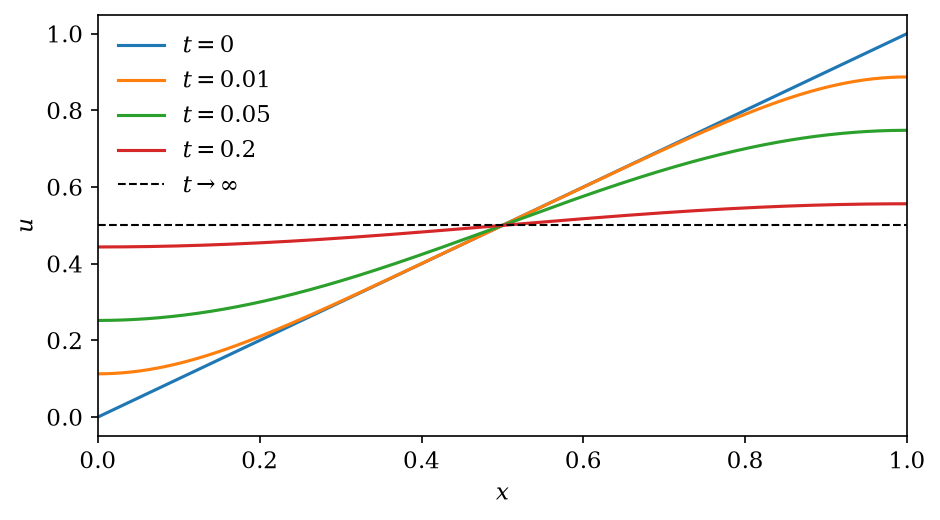
\includegraphics[width=0.75\textwidth]{p1}
\caption{Решение задачи 1 при $l=1$, $a=1$}
\label{fig:p1}
\end{figure}

\section{Задача 2}
Рассматриваем задачу 1 с неоднородными граничными условиями I рода на левом торце и II рода на правом, неоднородности постоянны:
\[
u_t=a^2u_{xx},\qquad u(x,0)=x,\qquad u(0,t)=A,\qquad -u_x(l,t)=B .
\]
Стационарный режим: $U''=0$, $U(0)=A$, $-U'(l)=B$, откуда
\[
U(x)=A-Bx .
\]
Проверим, что решение действительно стремится к $U$. Функция $v=u-U$ удовлетворяет
\[
v_t=a^2v_{xx},\qquad v(0,t)=0,\qquad v_x(l,t)=0,\qquad v(x,0)=(1+B)x-A .
\]
Решаем методом Фурье: ищем решения вида $v(x,t)=X(x)T(t)$. Как в п.~\ref{sec:green} (при $b=0$), получаем $X_n=\sin \lambda_nx$, $\lambda_n=\frac{(2n-1)\pi}{2l}$, $T_n=D_ne^{-a^2\lambda_n^2t}$. Коэффициенты $D_n$ находим из начального условия с помощью интегралов
\[
\frac2l\int_0^l\sin \lambda_nx\,dx=\frac{2}{l\lambda_n},\qquad \frac2l\int_0^lx\sin \lambda_nx\,dx=\frac{2(-1)^{n+1}}{l\lambda_n^2}
\]
получаем
\[
u(x,t)=A-Bx+\sum_{n=1}^{\infty}\Bigl(\frac{2(1+B)(-1)^{n+1}}{l\lambda_n^2}-\frac{2A}{l\lambda_n}\Bigr)e^{-a^2\lambda_n^2t}\sin \lambda_nx\ \xrightarrow[t\to\infty]{}\ A-Bx .
\]

\textbf{Зависимость от $A$ и $B$.} Стационарный режим~--- линейная функция, не зависящая от начальной температуры.
\begin{itemize}
\item $A$~--- температура левого торца; изменение $A$ сдвигает весь профиль на ту же величину.
\item $B=q_l/k$ пропорционален потоку через правый торец и задаёт наклон: при $B>0$ тепло уходит через правый торец и температура убывает к нему; при $B<0$ тепло поступает и температура возрастает; при $B=0$ правый торец теплоизолирован и $U\equiv A$.
\item Температура правого торца $U(l)=A-Bl$; $U\equiv0$ только при $A=B=0$.
\end{itemize}
\begin{figure}[H]
\centering
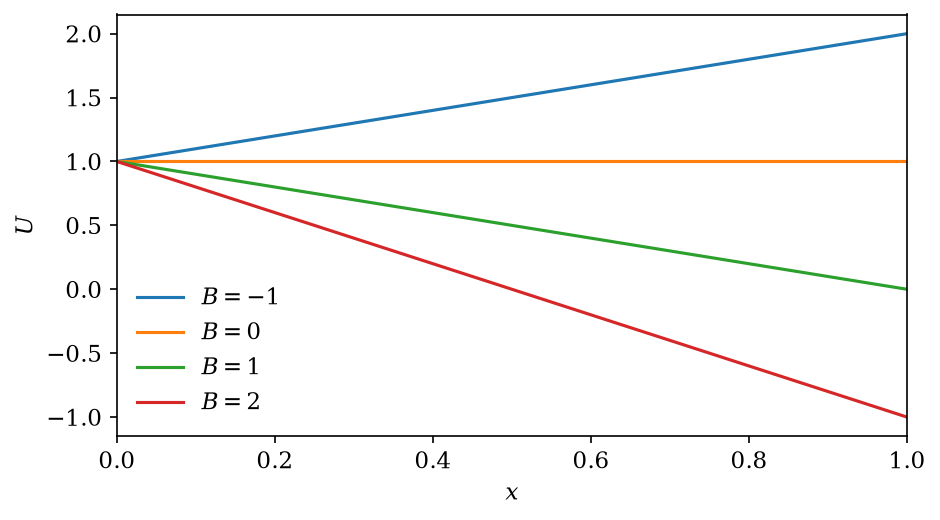
\includegraphics[width=0.75\textwidth]{p2}
\caption{Стационарный режим $U=A-Bx$ при $A=1$, $l=1$}
\label{fig:p2}
\end{figure}

\section{Задача 3}
Решаем задачу 1 ($b=0$, $f=0$, $\varphi=x$) с неоднородными граничными условиями:
\[
u_t=a^2u_{xx},\qquad u(x,0)=x,\qquad u(0,t)=\mu(t)=A\cos\omega_1t+B\sin\omega_2t,\qquad -u_x(l,t)=0 .
\]
\textbf{Устранение неоднородности.} Функция $w=\mu(t)$ удовлетворяет обоим граничным условиям. Положим $u=\mu(t)+v$:
\[
v_t=a^2v_{xx}-\mu'(t),\qquad v(0,t)=0,\qquad v_x(l,t)=0,\qquad v(x,0)=x-A .
\]
Ищем $v=\sum_{n=1}^\infty T_n(t)\sin p_nx$, $p_n=\frac{(2n-1)\pi}{2l}$, $\lambda_n=a^2p_n^2$. Раскладывая $1=\sum\frac{2}{lp_n}\sin p_nx$ и $x=\sum\frac{2(-1)^{n+1}}{lp_n^2}\sin p_nx$, получаем
\[
T_n'+\lambda_nT_n=-\frac{2}{lp_n}\mu'(t),\qquad T_n(0)=\frac{2(-1)^{n+1}}{lp_n^2}-\frac{2A}{lp_n},
\]
\[
T_n(t)=T_n(0)e^{-\lambda_nt}-\frac{2}{lp_n}\int_0^te^{-\lambda_n(t-\tau)}\mu'(\tau)\,d\tau .
\]
Для $\mu'(\tau)=-A\omega_1\sin\omega_1\tau+B\omega_2\cos\omega_2\tau$ нужны интегралы
\[
I_s(\lambda,\omega,t)=\int_0^te^{-\lambda(t-\tau)}\sin\omega\tau\,d\tau=\frac{\lambda\sin\omega t-\omega\cos\omega t+\omega e^{-\lambda t}}{\lambda^2+\omega^2},
\]
\[
I_c(\lambda,\omega,t)=\int_0^te^{-\lambda(t-\tau)}\cos\omega\tau\,d\tau=\frac{\lambda\cos\omega t+\omega\sin\omega t-\lambda e^{-\lambda t}}{\lambda^2+\omega^2}.
\]
Окончательно
\[
u(x,t)=A\cos\omega_1t+B\sin\omega_2t+\sum_{n=1}^{\infty}\Bigl[T_n(0)e^{-\lambda_nt}+\frac{2}{lp_n}\bigl(A\omega_1I_s(\lambda_n,\omega_1,t)-B\omega_2I_c(\lambda_n,\omega_2,t)\bigr)\Bigr]\sin p_nx .
\]

\textbf{Поведение при $t\to\infty$.} Все слагаемые с $e^{-\lambda_nt}$ затухают, начальная температура забывается. Остаются вынужденные колебания с частотами $\omega_1,\omega_2$. Их сумму можно записать в замкнутом виде (функция $e^{i\omega t}Y(x)$ с $a^2Y''=i\omega Y$, $Y(0)=1$, $Y'(l)=0$):
\[
u(x,t)\approx A\,\mathrm{Re}\Bigl[e^{i\omega_1t}\frac{\operatorname{ch}s_1(l-x)}{\operatorname{ch}s_1l}\Bigr]+B\,\mathrm{Im}\Bigl[e^{i\omega_2t}\frac{\operatorname{ch}s_2(l-x)}{\operatorname{ch}s_2l}\Bigr],\qquad s_j=(1+i)\sqrt{\frac{\omega_j}{2a^2}} .
\]
Амплитуда колебаний убывает от левого торца вглубь стержня, фаза запаздывает, тем сильнее, чем больше частота. Решение ограничено при любых вещественных $A,B,\omega_1,\omega_2$: так как $|\mu'|\le M=|A|\omega_1+|B|\omega_2$,
\[
\Bigl|\int_0^te^{-\lambda_n(t-\tau)}\mu'(\tau)d\tau\Bigr|\le\frac{M}{\lambda_n},\qquad
|u|\le|A|+|B|+\sum_{n}|T_n(0)|e^{-\lambda_nt}+M\sum_{n}\frac{2}{lp_n\lambda_n},
\]
а последний ряд сходится ($\sim1/n^3$).

\textbf{Подбор неоднородностей} (рис.~\ref{fig:p3}).
\begin{itemize}
\item \emph{Решение стремится к нулю}, если $A=B=0$ ($\mu\equiv0$). Тогда остаётся только $u=\sum\frac{2(-1)^{n+1}}{lp_n^2}e^{-\lambda_nt}\sin p_nx\to0$: тепло уходит через левый торец с нулевой температурой.
\item \emph{Решение стремится к константе}, если $\omega_1=0$, $B=0$, т.\,е. $\mu\equiv A$. Тогда в формуле остаются $A$ и затухающие слагаемые, $u\to A$; это задача 2 при $B=0$.
\item \emph{Неограниченное решение.} Как показано выше, при вещественных параметрах заданного вида решение ограничено. Неограниченность возникает при неограниченной неоднородности, например в пределе $\omega_2\to0$, $B\omega_2=C$, когда $B\sin\omega_2t\to Ct$. При $\mu=Ct$ имеем $\mu'=C$ и
\[
T_n=\frac{2(-1)^{n+1}}{lp_n^2}e^{-\lambda_nt}-\frac{2C}{lp_n\lambda_n}\bigl(1-e^{-\lambda_nt}\bigr),\qquad
u(x,t)\approx C\Bigl(t-\frac{x(2l-x)}{2a^2}\Bigr)\to\infty,
\]
где использовано $\sum\frac{2}{lp_n^3}\sin p_nx=\frac{x(2l-x)}{2}$.
\end{itemize}
\begin{figure}[H]
\centering
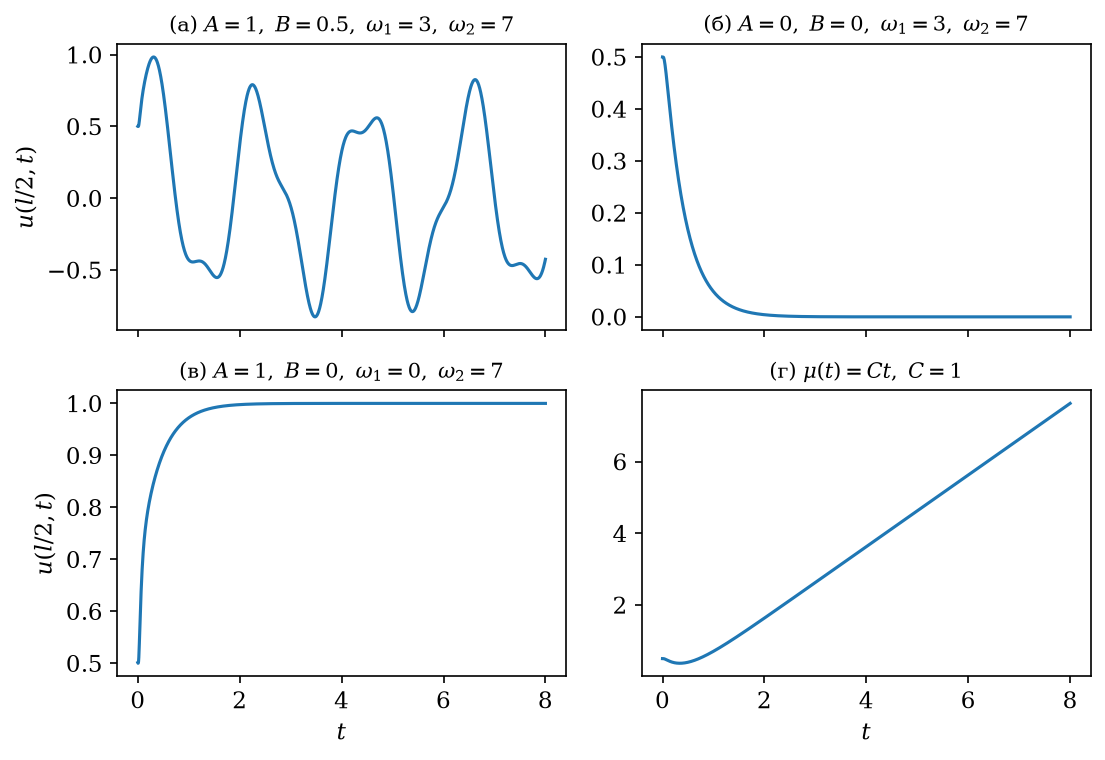
\includegraphics[width=0.95\textwidth]{p3}
\caption{Температура в середине стержня $u(l/2,t)$ при $l=1$, $a=1$: (а) общий случай; (б) $u\to0$; (в) $u\to A$; (г) неограниченный рост}
\label{fig:p3}
\end{figure}

\section{Задача 4}
Решаем задачу 2 при теплообмене через боковую поверхность со средой температуры $u_{\text{ср}}=\mathrm{const}$ (п.~\ref{sec:deriv}: $b=\frac{hP}{c\rho S}>0$, $f=bu_{\text{ср}}$):
\[
u_t=a^2u_{xx}-b(u-u_{\text{ср}}),\qquad u(x,0)=x,\qquad u(0,t)=A,\qquad -u_x(l,t)=B .
\]
Обозначим $\kappa=\sqrt b/a$.

\textbf{Температура среды равна нулю} ($u_{\text{ср}}=0$). Стационарный режим: $U''-\kappa^2U=0$, $U(0)=A$, $U'(l)=-B$. Из $U=C_1\operatorname{ch}\kappa x+C_2\operatorname{sh}\kappa x$ находим $C_1=A$, $C_2=-\frac{A\operatorname{sh}\kappa l+B/\kappa}{\operatorname{ch}\kappa l}$, т.\,е.
\[
U_0(x)=\frac{A\operatorname{ch}\kappa(l-x)-\frac B\kappa\operatorname{sh}\kappa x}{\operatorname{ch}\kappa l}.
\]

\textbf{Температура среды постоянна.} Замена $u=u_{\text{ср}}+w$ приводит к случаю $u_{\text{ср}}=0$ для $w$ с $A$, заменённым на $A-u_{\text{ср}}$ ($B$ не меняется), поэтому
\[
U(x)=u_{\text{ср}}+\frac{(A-u_{\text{ср}})\operatorname{ch}\kappa(l-x)-\frac B\kappa\operatorname{sh}\kappa x}{\operatorname{ch}\kappa l}.
\]

\textbf{Полное решение.} Функция $v=u-U$ решает задачу $v_t=a^2v_{xx}-bv$, $v(0,t)=0$, $v_x(l,t)=0$, $v(x,0)=x-U(x)$, поэтому $v=\sum D_ne^{-(a^2p_n^2+b)t}\sin p_nx$. Коэффициенты $U$ находим, умножая $U''=\kappa^2(U-u_{\text{ср}})$ на $\sin p_nx$ и дважды интегрируя по частям:
\[
\frac2l\int_0^lU\sin p_nx\,dx=\frac2l\cdot\frac{Ap_n+(-1)^nB+\kappa^2u_{\text{ср}}/p_n}{p_n^2+\kappa^2}.
\]
Итак,
\[
u(x,t)=U(x)+\sum_{n=1}^{\infty}\Bigl(\frac{2(-1)^{n+1}}{lp_n^2}-\frac2l\cdot\frac{Ap_n+(-1)^nB+\kappa^2u_{\text{ср}}/p_n}{p_n^2+\kappa^2}\Bigr)e^{-(a^2p_n^2+b)t}\sin p_nx .
\]
При $b=0$ ($\kappa\to0$) формула переходит в решение задачи 2.

\textbf{Анализ.} Решение стремится к $U$, причём быстрее, чем в задаче 2: показатели затухания увеличились на $b$. С ростом $b$ профиль отходит от прямой $A-Bx$ и внутри стержня приближается к температуре среды $u_{\text{ср}}$; отличие от $u_{\text{ср}}$ сохраняется в слое толщины порядка $1/\kappa$ у левого торца, где поддерживается температура $A$ (рис.~\ref{fig:p4}). Температура правого торца
\[
U(l)=u_{\text{ср}}+\frac{A-u_{\text{ср}}-\frac B\kappa\operatorname{sh}\kappa l}{\operatorname{ch}\kappa l}.
\]
При $u_{\text{ср}}=0$ и $B>0$ она может стать отрицательной: тепло уходит и через боковую поверхность, и через правый торец.
\begin{figure}[H]
\centering
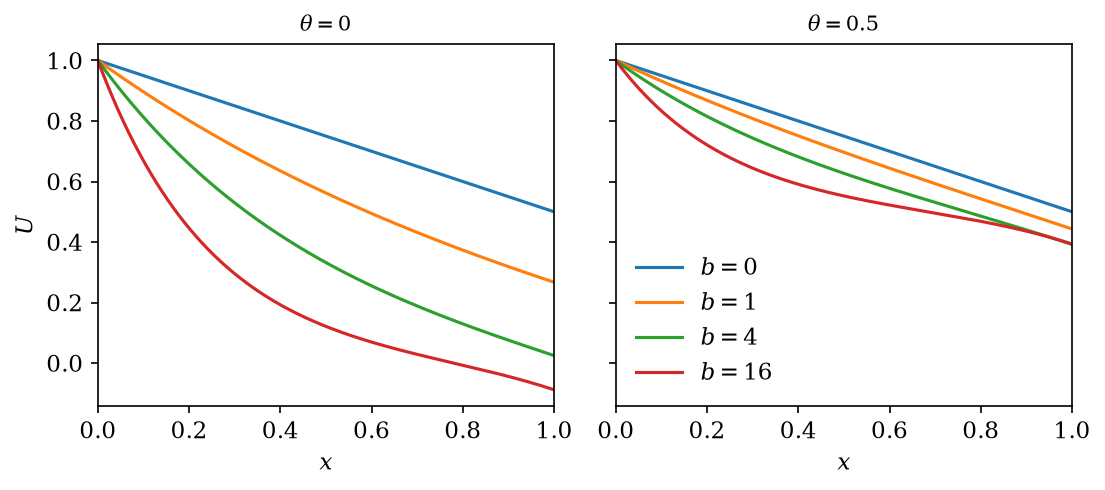
\includegraphics[width=0.95\textwidth]{p4}
\caption{Стационарный режим задачи 4 при $A=1$, $B=0.5$, $l=1$, $a=1$}
\label{fig:p4}
\end{figure}

\section{Задача 5}
Температура шара зависит только от $r$ и $t$. В сферических координатах
\[
u_t=a^2\Bigl(u_{rr}+\frac2ru_r\Bigr),\quad 0\le r<R,\qquad u(r,0)=0,\qquad k\,u_r(R,t)=q,\qquad |u(0,t)|<\infty .
\]
Граничное условие получено так же, как в п.~\ref{sec:deriv}: поток, входящий через поверхность, равен $k\,\partial u/\partial n=k\,u_r$.

\textbf{Выделение растущей части.} Всё подводимое тепло остаётся в шаре, поэтому средняя температура растёт линейно: $c\rho\frac43\pi R^3\bar u=4\pi R^2qt$, т.\,е. $\bar u=\frac{3a^2q}{kR}t$. Ищем $u=\frac{3a^2q}{kR}t+g(r)+v(r,t)$. Для $g$:
\[
a^2\Bigl(g''+\frac2rg'\Bigr)=\frac{3a^2q}{kR},\qquad k\,g'(R)=q\quad\Rightarrow\quad g=\frac{q}{k}\Bigl(\frac{r^2}{2R}-\frac{3R}{10}\Bigr),
\]
где константа выбрана так, что $\int_0^Rg\,r^2dr=0$. Тогда $v$ решает однородную задачу
\[
v_t=a^2\Bigl(v_{rr}+\frac2rv_r\Bigr),\qquad v_r(R,t)=0,\qquad v(r,0)=-g(r).
\]

\textbf{Метод Фурье.} Замена $v=w/r$ даёт $w_t=a^2w_{rr}$, $w(0,t)=0$, $Rw_r(R,t)-w(R,t)=0$. Ищем решения вида $w(r,t)=X(r)T(t)$:
\[
X''+\lambda X=0,\quad X(0)=0,\quad RX'(R)-X(R)=0,\qquad T'+a^2\lambda T=0 .
\]
Из $X(0)=0$ следует $X=\sin\sqrt\lambda r$, а условие при $r=R$ с $\mu=\sqrt\lambda R$ даёт $\mu\cos\mu-\sin\mu=0$. Собственные функции $\sin\frac{\mu_nr}{R}$, $T_n=e^{-a^2\mu_n^2t/R^2}$, где $\mu_n$~--- положительные корни уравнения
\[
\operatorname{tg}\mu=\mu\qquad(\mu_1\approx4.4934,\ \mu_2\approx7.7253,\ \mu_3\approx10.9041,\dots),
\]
и $\int_0^R\sin^2\frac{\mu_nr}{R}dr=\frac R2\sin^2\mu_n$. Значению $\mu=0$ соответствует постоянная $v$, но её коэффициент равен нулю, так как среднее $g$ равно нулю. Коэффициенты разложения $-rg(r)$:
\[
D_n=-\frac{\int_0^Rrg(r)\sin\frac{\mu_nr}{R}dr}{\frac R2\sin^2\mu_n}=-\frac{2qR^2}{k\mu_n^2\sin\mu_n},
\]
где интеграл $\int_0^Rrg\sin\frac{\mu_nr}{R}dr=\frac{qR^3\sin\mu_n}{k\mu_n^2}$ вычислен двукратным интегрированием по частям с учётом $\operatorname{tg}\mu_n=\mu_n$.

\textbf{Ответ.}
\[
u(r,t)=\frac qk\Bigl(\frac{3a^2t}{R}+\frac{5r^2-3R^2}{10R}\Bigr)-\frac{2qR^2}{k\,r}\sum_{n=1}^{\infty}\frac{\sin\frac{\mu_nr}{R}}{\mu_n^2\sin\mu_n}\,e^{-\frac{a^2\mu_n^2}{R^2}t},\qquad \operatorname{tg}\mu_n=\mu_n .
\]
В центре шара $\frac1r\sin\frac{\mu_nr}{R}\to\frac{\mu_n}{R}$. При больших $t$ ряд затухает, температура растёт линейно со скоростью $\frac{3a^2q}{kR}=\frac{3q}{c\rho R}$, а её распределение по радиусу сохраняет параболическую форму: поверхность горячее центра на $\frac{qR}{2k}$ (рис.~\ref{fig:p5}).
\begin{figure}[H]
\centering
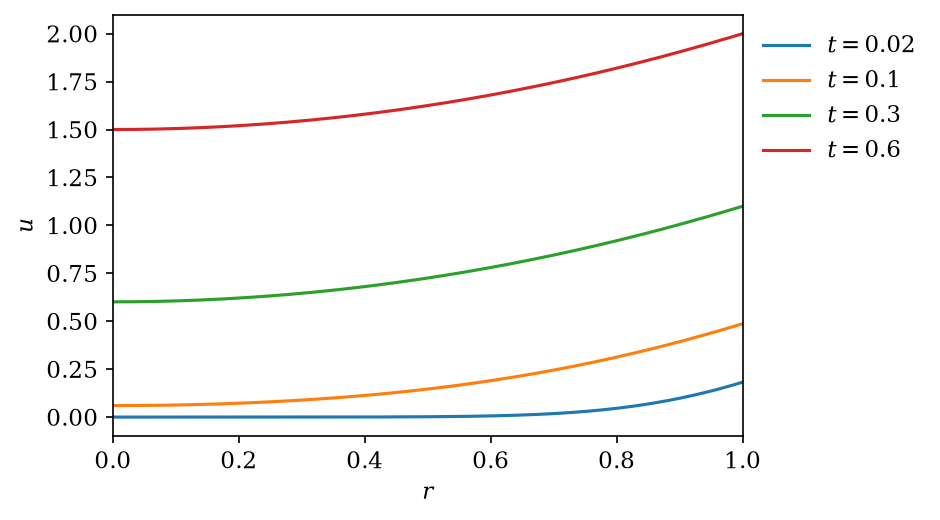
\includegraphics[width=0.75\textwidth]{p5}
\caption{Распределение температуры в шаре при $R=1$, $a=1$, $q/k=1$}
\label{fig:p5}
\end{figure}

\end{document}
